\subsection{Ejemplo completo de Lógica Combinacional}
Un detector de paridad impar de 4 entradas y una salida funciona de la siguiente manera: si la cantidad de entradas con valor ‘1’ es impar la salida se pone en ‘1’, en el resto de los casos la salida toma valor ‘0’.
\begin{enumerate}%[label=\alph*), labelindent=1em]
    \item Construir la tabla de verdad para dicho sistema.
    \item Obtener la ecuación lógica como suma de minitérminos y producto de maxitérminos (funciones canónicas).
    \item Implementar el sistema con compuertas NAND de la cantidad de entradas requeridas.
    \item Implementar el sistema con una PLA.
\end{enumerate}

\subsection*{Punto 1}
Para construir la tabla de verdad, se deben considerar las 4 entradas posibles y la salida que se obtiene para cada combinación de entradas.

\begin{table}[h]
    \centering
    \begin{tabular}{cccc|c|c|c}
        \toprule
        \textbf{A} & \textbf{B} & \textbf{C} & \textbf{D} & \textbf{S} & \textbf{Minitérminos} & \textbf{Maxitérminos}\\
        \midrule
        0 & 0 & 0 & 0 & 0 & $m_0$ = A'B'C'D' & $M_0$ = A+B+C+D\\
        0 & 0 & 0 & 1 & 1 & $m_1$ = A'B'C'D & $M_1$ = A+B+C+D'\\
        0 & 0 & 1 & 0 & 1 & $m_2$ = A'B'CD' & $M_2$ = A+B+C'+D\\
        0 & 0 & 1 & 1 & 0 & $m_3$ = A'B'CD & $M_3$ = A+B+C'+D'\\
        0 & 1 & 0 & 0 & 1 & $m_4$ = A'BC'D' & $M_4$ = A+B'+C+D\\
        0 & 1 & 0 & 1 & 0 & $m_5$ = A'BC'D & $M_5$ = A+B'+C+D'\\
        0 & 1 & 1 & 0 & 0 & $m_6$ = A'BCD' & $M_6$ = A+B'+C'+D\\
        0 & 1 & 1 & 1 & 1 & $m_7$ = A'BCD & $M_7$ = A+B'+C'+D'\\
        1 & 0 & 0 & 0 & 1 & $m_8$ = AB'C'D' & $M_8$ = A'+B+C+D\\
        1 & 0 & 0 & 1 & 0 & $m_9$ = AB'C'D & $M_9$ = A'+B+C+D'\\
        1 & 0 & 1 & 0 & 0 & $m_{10}$ = AB'CD' & $M_{10}$ = A'+B+C'+D\\
        1 & 0 & 1 & 1 & 1 & $m_{11}$ = AB'CD & $M_{11}$ = A'+B+C'+D'\\
        1 & 1 & 0 & 0 & 0 & $m_{12}$ = ABC'D' & $M_{12}$ = A'+B'+C+D\\
        1 & 1 & 0 & 1 & 1 & $m_{13}$ = ABC'D & $M_{13}$ = A'+B'+C+D'\\
        1 & 1 & 1 & 0 & 1 & $m_{14}$ = ABCD' & $M_{14}$ = A'+B'+C'+D\\
        1 & 1 & 1 & 1 & 0 & $m_{15}$ = ABCD & $M_{15}$ = A'+B'+C'+D'\\
        \bottomrule
    \end{tabular}
\end{table}

\subsection*{Punto 2}
Para obtener la ecuación lógica como suma de minitérminos y producto de maxitérminos, se deben identificar los términos que hacen que la función devuelva $1$ y los términos que hacen que la función devuelva $0$.

\begin{itemize}
    \item \textbf{Suma de minitérminos:} tomo los términos que hacen 1 la función y los sumo.
    \begin{equation*}
        F = m_1 + m_2 + m_4 + m_7 + m_8 + m_{11} + m_{13} + m_{14}
    \end{equation*}
    Desarrollando la ecuación, se obtiene:
    \begin{equation*}
        F = A'B'C'D + A'B'CD' + A'BC'D' + A'BCD + AB'C'D' + AB'CD + ABC'D + ABCD'
    \end{equation*}

    \item \textbf{Producto de maxitérminos:} tomo los términos que hacen 0 la función y los multiplico.
    \begin{equation*}
        F = M_0 \cdot M_3 \cdot M_5 \cdot M_6 \cdot M_9 \cdot M_{10} \cdot M_{12} \cdot M_{15}
    \end{equation*}
    Desarrollando la ecuación, se obtiene:
    \begin{align*}
        F &= (A+B+C+D)(A+B+C'+D')(A+B'+C+D')(A+B'+C'+D)(A'+B+C+D') \\
        & (A'+B+C'+D')(A'+B'+C+D)(A'+B'+C'+D')
    \end{align*}
\end{itemize}

\subsection*{Punto 3}
Para implementar el sistema con compuertas NAND, se deben seguir los siguientes pasos:
\begin{enumerate}
    \item Se toma la forma canónica de la función lógica, en este caso se tomará la forma de suma de minitérminos.
    \item Luego se niega dos veces la función lógica, para obtener la forma de producto de maxitérminos.
    \item Se aplica una vez más la ley de De Morgan para obtener la forma buscada.
\end{enumerate}

\begin{align*}
    F &= A'B'C'D + A'B'CD' + A'BC'D' + A'BCD + AB'C'D' + AB'CD + ABC'D + ABCD' \\
    &= (A'B'C'D + A'B'CD' + A'BC'D' + A'BCD + AB'C'D' + AB'CD + ABC'D + ABCD')'' \\
    &= (A'B'C'D)' \cdot (A'B'CD')' \cdot (A'BC'D')' \cdot (A'BCD)' \cdot (AB'C'D')' \cdot (AB'CD)' \cdot (ABC'D)' \cdot (ABCD')'
\end{align*}

\subsection*{Punto 4}
Para implementar el sistema con una PLA, se utilizará la forma canónica de la función lógica, en este caso se tomará la forma de suma de minitérminos.

\begin{figure}[h]
    \centering
    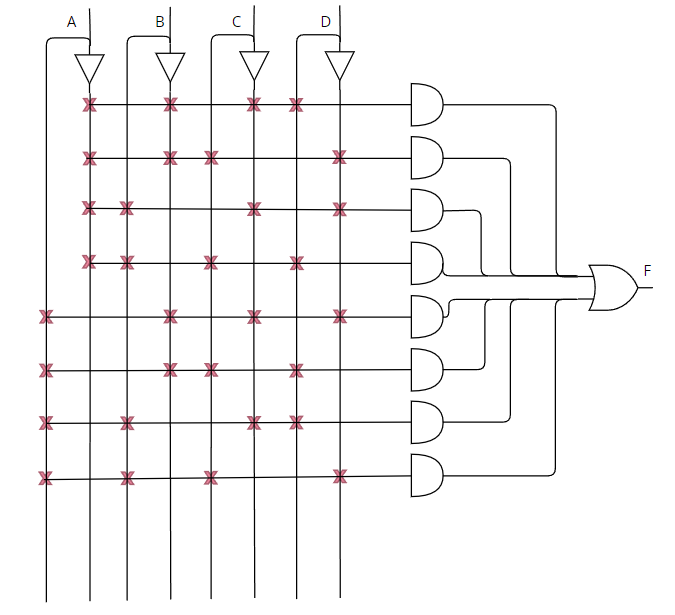
\includegraphics[scale=0.65]{img/plaej.png}
    \caption{Estructura de la función lógica en una PLA.}
\end{figure}